\chapter{Підходи до формалізації голосової взаємодії в системі диспетчеризації} \label{chapt2}

\section{Концепція створення системи автоматизації голосової взаємодії} \label{sect2_1}

У результаті аналізу виявлено два найбільш перспективні напрями, поєднання яких дає змогу запропонувати нове принципове рішення і побудувати рефлекторну модель голосової взаємодії в задачах управління дистрибуцією. В основу моделі покладено логічні сценарії взаємодії на тему управління дистрибуцією, які мають враховувати параметри основних причин невідповідності реальної ситуації запланованому маршруту, наприклад, запізнення або відмови обслуговування на точці доставки тощо. Це дає змогу отримати інформацію для прийняття рішення про повернення вантажу на склад, про відміну чи відкладення обслуговування однієї точки доставки, щоб мати можливість встигнути на іншу, більш важливу, про зміну маршруту для обʼїзду затору або про утворення нового маршруту з резервною машиною тощо.

Звичайно, абсолютно всі причини та параметри не можуть бути враховані заздалегідь, але проробка і врахування основної типології дозволить приймати базові рішення та вдаватися до безпосереднього звʼязку з диспетчером лише у складних випадках, що розвантажить водія та канали комунікації і дасть змогу підвищити загальну ефективність дистрибуції.

Найбільш ефективним шляхом розробки дерева сценаріїв рефлекторної взаємодії є використання вхідних параметрів вже створеної системи автоматизації дистрибуції, у тому числі автоматичної побудови маршрутів \cite{as6}, яка зараз проходить широку експериментальну апробацію. Інтеграція модулю голосової взаємодії з цією системою буде значно спрощена, що сприятиме отриманню кращого економічного ефекту.

Виходячи з наявної логіки побудови маршрутів, вже зараз можна назвати принципові блоки сценаріїв, які потрібно буде розробити. Першим етапом, на якому можуть виникнути проблеми розбіжності плану та факту, є етап завантаження на складі (якщо, наприклад, буде виявлений неврахований «перегруз» або «недогруз» машини, будуть відсутні необхідні товари чи працівники складу не встигнуть їх вчасно відібрати, або навіть виявиться, що машина не здатна вийти на маршрут (наприклад, не заводитися на морозі)).

Другий етап сценаріїв голосової взаємодії визначають проблеми, які можуть виникнути в дорозі до певної точки доставки, як, наприклад, ремонт в дорозі по маршруту руху або зміни в правилах руху на деяких вулицях, які ще не відбиті в алгоритмах прокладення маршруту (нові заборони поворотів чи односторонній рух), проблеми з автомобілем на дорозі, які призводять до зниження швидкості або відмови в подальшому русі по маршруту, або найбільш розповсюджена проблема заторів на дорогах. 

Третій етап сценаріїв голосової взаємодії викликаний можливими невідповідностями між планом та фактом в обслуговуванні на точці доставки. Це можуть бути як проблеми зі сторони клієнта («нікого немає вдома», клієнт не має грошей, клієнт відмовляється від замовлення чи стверджує, що він замовляв щось інше), так і проблеми зі сторони водія (запізнення на точку доставки, тобто не потрапляння в заплановане дозволене часове вікно доступності, пошкодження товару тощо). Найбільш поширеною є ситуація, коли водій проводить в точці доставки більше часу, ніж заплановано, що призводить до проблем на всьому подальшому маршруті.

Ці та інші інциденти на всіх зазначених етапах, що зазначені в моделі на схемі (рис. \ref{img:voice_interaction_schema}), потребують вирішення із залученням диспетчера для вибору найкращої стратегії і мінімізації втрат через проблему. Відповідно дерево сценаріїв голосової взаємодії повинно відбивати всі три етапи та типові відомі проблеми і способи їх розвʼязання.

\begin{figure}
	\centering
	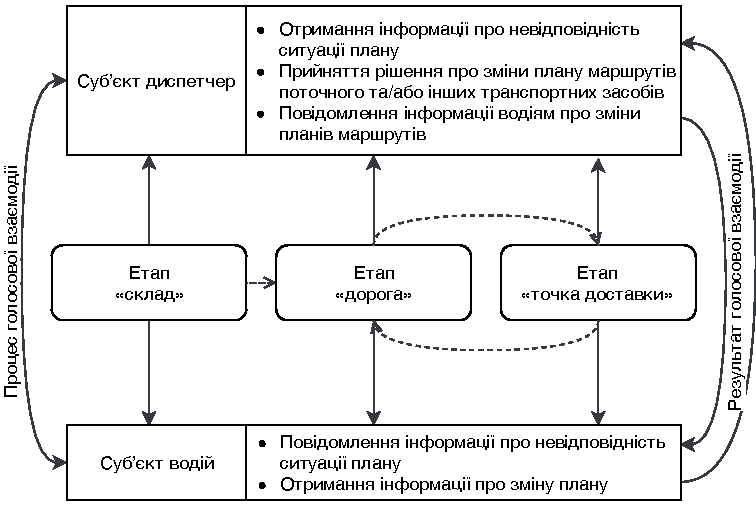
\includegraphics [width=\linewidth] {voice_interaction_schema}
	\caption{Схема голосової взаємодії субʼєктів дистрибуції}
	\label{img:voice_interaction_schema}
\end{figure}

Схема голосової взаємодії субʼєктів дистрибуції зображена на рис. \ref{img:voice_interaction_schema}. Вона складається з трьох етапів, два останніх з яких, можуть циклічно повторюватися при наявності декількох точок доставки в маршруті. Стрілками позначено процеси голосової взаємодії, які можуть розгортатися на кожному з етапів при невідповідності плану та факту. У верхній та нижній частинах схеми показані принципові типи результатів голосової взаємодії для кожного з субʼєктів (диспетчера та водія). Ця логічна схема визначає принциповий алгоритм побудови дерева сценаріїв голосової взаємодії.

Другим важливим та перспективним напрямом, який дає змогу побудувати рефлекторну модель голосової взаємодії в задачах управління дистрибуцією, є застосування рефлекторних систем голосового управління. Ідея, покладена в основу цього підходу, полягає в тому, щоб замість переведення голосової інформації в текстову репрезентацію, аналізувати безпосередньо інформаційну складову сказаного, визначаючи, яку з відомих реакцій потрібно виконати. «Традиційні системи розпізнавання мови засновані на принципі: „усна мова“ → „репрезентація мови набором лінгвістичних конструкцій“ → „розуміння мови“. На основі теорії несиловой взаємодій може бути запропонована інша модель розпізнавання природної мови: „усна мова“ → „розрахунок несилової (інформаційної) взаємодії на реакції“ → „реакція (розуміння чи поведінка)“» \cite{Teslia_2014}.

Тобто така система буде складатися з двох основних компонентів (рис. \ref{img:rgsu_concept}). Перший компонент --- розпізнавання мови, це може бути будь-яка система переведення голосового сигналу в текстову репрезентацію --- як лексичну так і фонетичну. В нашій роботі ми будемо використовувати фонетичну текстову репрезентацію, оскільки її створення не потребує наявності великих контекстно-залежних словників, що більше підходить для використання на мобільному пристрої з обмеженим доступом до мережі інтернет.

\begin{figure}
	\centering
	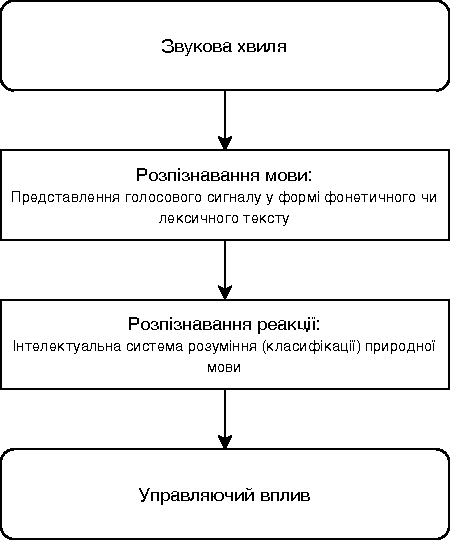
\includegraphics [width=.5\linewidth] {rgsu_concept}
	\caption{Схема узагальненої структури рефлекторних систем голосового управління}
	\label{img:rgsu_concept}
\end{figure}

Другий компонент --- розпізнавання реакції по розпізнаній мові. Концептуально це може бути будь-яка інтелектуальна система розуміння (класифікації) природної мови. В нашій роботі ми будемо розглядати метод інтелектуальних рефлекторних систем, оскільки його ефективність в роботі з фонетичним текстом вже була доведена і метод згорткових нейронних мереж, оскільки вони показали гарні результати при роботі з лексичним текстом посимвольно, що є найбільш схоже на роботу з фонетичним текстом.

\section{Методи автоматизації руху автотранспорту в дистрибуції та параметри що впливають на сценарії голосової взаємодії} \label{sect2_2}

Транспортна логістика --- це система організації доставки, а саме переміщення будь-яких матеріальних предметів або речовин з однієї точки в іншу за оптимальним маршрутом. Транспортна логістика є частиною процесів дистрибуції, курʼєрської доставки, та інших транспортних систем, що включають в себе перевезення вантажів. Важливим етапом в процесах транспортної логістики є так званий етап «останньої милі» --- останній етап доставки вантажу з розподільчого центру до клієнта. Цей етап найменш ефективний з усього ланцюгу поставок, і може коштувати до 28\% від усієї вартості доставки. \cite{Scott_2009}

Для транспортної логістики на етапі останньої милі дуже важливим є планування маршрутів, а також моніторинг та диспетчеризація процесу доставки. Адже якісний маршрут дозволяє зменшити транспортні витрати, а моніторинг --- підвищує рівень сервісу в реакціях на позапланові ситуації. 

На жаль сьогодні в більшості компаній України планування відбувається на достатньо примітивному рівні --- логісти визначають який транспортний засіб повезе який вантаж, але не створюють конкретний маршрут, залишаючи це рішення на водіїв. Це повʼязано в першу чергу з тим що логісти розробляють планові маршрути вручну без залучення автоматизованих систем. Друга причина, що випливає з першої --- логісти не можуть гарантувати принципову виконуваність маршрутів, оскільки орієнтуються в більшій мірі на масо-габаритні параметри, а часові вимоги враховують лише частково. Адже масо-габаритні параметри можна порахувати сумарно незалежно від порядку обʼїзду точок доставки, а часові параметри можливо перевірити лише для конкретного маршруту, побудова і розрахунок якого виходить за межі людських можливостей без використання технічних засобів. Оскільки набір точок доставки для кожного окремого транспортного засобу не є гарантовано виконуваним, то розраховувати маршрути окремих транспортних засобів не має сенсу --- потрібно вирішувати задачу в цілому для всіх точок доставки та машин, що відноситься до суттєво складнішого класу задач --- Vehicle Routing Problem (VRP).

Запровадження автоматичного розрахунку маршрутів несе в собі декілька суттєвих переваг. По перше це гарантованість принципової виконуваності маршрутів, без урахування позапланових ситуацій. По друге це підвищення рівня сервісу, адже маючи конкретний маршрут з плановим часом прибуття, ми можемо повідомити його клієнту, скоротивши його час очікування. Наприклад якщо клієнт замовив доставку з 15:00 до 18:00, він не буде 3 години <<сидіти на стільці>> в очікуванні доставки --- він в цей час лише переважно буде знаходитися в місці доставки, але буде займатися своїми справами, можливо на щось відволічіться чи відійде на короткий час. Якщо ми повідомимо клієнту орієнтовний час доставки (наприклад з 17:00 по 17:30), то ми забезпечимо клієнту більшу свободу дій, та знизимо ймовірність того, що саме в час прибуття доставки, клієнт не зможе її прийняти вчасно, що призведе до затримки.

По третє наявність планового маршруту підвищить можливості моніторингу та реакції на позапланові ситуації. Без планового маршруту, за допомогою GPS моніторингу можливо лише побачити де перебував транспортний засіб та де він зупинявся. Але оскільки невідомий план за яким рухається водій, не зрозуміло, чи зупинка означає обслуговування точки доставки, чи водій відклав цю точку пізніше за планом і просто проїжджав повз, а зупинка --- наприклад, очікування світлофора. Крім того, не маючи плану руху транспортного засобу, не можна спрогнозувати, чи курʼєр встигає обслуговувати усі точки доставки вчасно --- можливо побачити лише факт того що якась із точок не відвідана, а замовлений клієнтом час уже вийшов. Маючи плановий маршрут, можливо в кожний момент часу спрогнозувати приблизний час прибуття на кожну з наступних точок із урахуванням можливого відставання, і побачити чи не призводить це відставання до порушення замовлених клієнтом часових вікон в майбутньому. Маючи цю інформацію набагато легше прийняти своєчасні дії --- повідомити водію про необхідність пришвидшити обслуговування точок або обговорити з клієнтом можливість перенесення часу доставки.

Варто не відкидати також і можливу економію за рахунок покращення ефективності планових маршрутів після запровадження автоматизованого планування. Тим не менше практика показує, що водій, який добре знає ввірену йому територію планує свій маршрут на достатньо високому рівні. Іноді рівень який може забезпечити водій з досвідом роботи навіть кращий за автоматизовані рішення, за рахунок наявності більш детальної інформації про карту району. Тим не менше автоматизоване планування може відвʼязати якість маршрутів від людського фактору --- рівня досвіду кожного конкретного водія.

Точне вирішення задачі маршрутизації транспортних засобів неможлива для розмірів задач, з якими стикаються сучасні курʼєрські служби в містах-мегаполісах. Навіть не всі евристичні алгоритми можуть задовольнити сучасні потреби у швидкості обрахунку. В залежності від бізнес-процесів конкретної компанії та організації системи обліку та контролю за помилками, бувають ситуації коли остаточна інформація про наявні замовлення отримується лише після прибуття вантажу на розподільчий пункт і часу на планування, завантаження та відправлення курʼєрів залишається дуже мало, тому час розрахунку стандартної задачі в 2--3 тисячі точок доставки не може займати більше 30--40 хвилин.

Основна проблема впровадження систем побудови планових маршрутів на практиці полягає у спротиві інноваціям на рівні кінцевих виконавців. Водії, особливо, якщо це наймані перевізники, а не співробітники компанії, відмовляються їхати по запропонованим програмою маршрутам. Перевізників не дуже хвилює глобальна оптимальність всіх маршрутів чи рівень сервісу кінцевого клієнта, якщо до цих параметрів не привʼязана їх платня. Вони звикли отримувати маршрутний лист сформований лише за територіальними та масо-габаритними критеріями, а до часових обмежень кінцевих клієнтів ставитися доволі формально. Тому будь-які зміни звичних планів сприймаються дуже негативно, аж до саботування всього процесу. Навіть в ідеально правильному рішенні може бути необхідність заїхати на територію іншого водія для доставки в деякі точки, які інший водій не встигне виконати або необхідність доставляти точки в районі який водій погано знає, оскільки його знайомому районі в певний день мале навантаження і він може весь бути обслугований сусідами без участі цього водія, а в іншому місці навпаки навантаження велике і потрібно залучення додаткових машин. Але більшість наявних евристик орієнтуються лише на сумарну вартість, і може робити подібного роду помилки в формуванні окремого маршруту, навіть коли в цьому немає нагальної необхідності.

Таким чином постає необхідність розробки евристичного алгоритму який би максимально враховував вимоги логістів та водіїв, щодо оптимальності вибору точок з точки зору кожного конкретного маршруту, при цьому не відкидаючи глобальну оптимальність при високій швидкості обрахунку.

Практика показує, що одним з найбільш визначальних вхідних параметрів, що може сильно вплинути на результат планування та можливість його втілення у  реальність, є кількість часу, що запланована на обслуговування в точок. Адже інші параметри визначені достатньо чітко - масо-габаритні параметри відомі заздалегідь, дозволені часові вікна визначає кінцевий клієнт. Для визначення часу та відстані руху по дорозі між двома точками, є багато вже розроблених інструментів, які прогнозують результат з достатнім рівнем похибки на основі статистичних даних. Але для визначення часу обслуговування точки немає достовірного джерела інформації: ані клієнт, ані водій, ані логіст не можуть його назвати. Найбільш розповсюджена помилка --- писати всім точкам однаковий час, наприклад 10 чи 5  хвилин, незалежно від ваги та кількості вантажу який необхідно доставити або складності пошуку та підʼїзду до точки доставки. Кращий варіант, який можна зустріти доволі часто - категоризація точок або конкретних замовлень, використовувати фіксований час обслуговування для всіх замовлень в категорії. Найбільш правильним варіантом, що може принести суттєву економію транспортного ресурсу при побудові планових маршрутів, є статистичний аналіз історії часу обслуговування точок. Моделювати кількість часу необхідного для виконання точки, потрібно виходячи з наступних параметрів: скільки часу використовувалося на обслуговування цієї та схожих точок в минулому, якими водіями та на яких машинах вони при цьому обслуговувалися, яку вагу, обʼєм та кількість вантажу було доставлено, та інші. Питання вибору оптимального способу моделювання заслуговує окремого дослідження.

Тим не менше, для подібного статистичного аналізу, постає проблема збору цих історичних даних. Достатньо точно час зупинки можна визначити за допомогою аналізу GPS треку, але цей метод має ряд недоліків. По перше, GPS дані мають похибку, яка може збільшуватись як в залежності від якості апаратного забезпечення, так і в залежності від території що обслуговується. Наприклад відомо що зонах висотної забудови GPS сигнал істотно погіршується, а іноді навіть втрачається повністю. Таке погіршення сигналу може згубно впливати на визначення часу зупинки або навіть факту зупинки взагалі. По друге, навіть якщо відкинути похибку GPS як не суттєву або прийнятну, постає питання співвідношення зупинок та точок доставки. У загальному випадку таке співвідношення однозначно можливе тільки якщо в заданому радіусі є лише одна зупинка та одна точка доставки. У випадках коли зупинка відбулася поза заданим радіусом, коли біля точки було кілька зупинок (в тому числі з причин хибної інтерпретації зупинки через похибки GPS), або, як це трапляється найчастіше, одна зупинка знаходиться близько до декількох точок, --- однозначно співвіднести з якої з зупинок необхідно записати час обслуговування точки неможливо. В сучасному світі, в містах мегаполісах, ситуація коли необхідно зробити декілька доставок в один багатоквартирний будинок, або сусідні будинки зі спільним двором, відбувається достатньо часто, і це автоматично унеможливлює збір та аналіз великої частини статистичної інформації про час обслуговування точки на основі GPS даних.

Отже необхідно доповнити дані GPS додатковою інформацією про те, коли водій-експедитор закінчив виконання однієї з точок в межах єдиної зупинки і почав виконання наступної точки. Практика показує що спроби зобовʼязати водія в цей момент діставати телефон/планшет і вибирати відповідну команду в мобільному додатку експедитора, у кращому випадку призводить лише до того, що водій відмітить всі точки як виконані ще до або вже після виконання всіх доставок на зупинці, адже маніпуляції з планшетом потребують часу, а руки в цей момент зазвичай зайняті. Для вирішення цієї проблеми потрібен зручний для водія/експедитора інтерфейс, який би не відволікав його від основного завдання. Таким може виступати голосовий інтерфейс, який буде сприймати команди про початок та завершення виконання доставки.


\section{Методи представлення дерева сценаріїв взаємодії з урахуванням не голосової інформації} \label{sect2_3}

Для представлення дерева сценаріїв найкраще підходить орієнтований граф, в якому вершини позначають стан системи та діалогові фрази які буде озвучувати система, а ребра --- репліки (стимулів) які можуть бути сприйняті системою в кожній конкретній вершині. Реакція на стимул може привести до переходу між станами, отже орієнтоване ребро проводиться від тієї вершини в якій стимул може бути сприйнятий, до тієї, в який стан система перейде в якості реакції на стимул. Отже множина всіх ребер, що виходять з вершини, позначають перелік стимулів, між якими треба проводити розпізнання для стану, що відповідає цей вершині.

Назва «дерево» сценаріїв використовується як сталий вираз, але реально представити всю необхідну інформацію у вигляді дерева неможливо, адже переходи між станами неминуче приводять до утворення циклів, а отже граф для представлення такої інформації підходить краще.

На жаль такій схемі недостатньо повноти для представлення всіх можливих варіантів перебігу подій. По перше реакції системи не обмежуються переключенням станів (контекстів) що позначають доступний перелік стимулів та відтворенням діалогових фраз. Основне корисне навантаження системи --- комунікація між водієм і диспетчером та керування процесом доставки, а отже нам необхідний спосіб представлення інших реакцій на стимули, таких як відправлення певної інформації в диспетчерський центр, отримання інструкцій з диспетчерського центру, переключення внутрішніх змінних для можливості повідомити водію контекстно-залежну інформацію про "поточну" точку доставки, тощо.

По друге стимули які можуть викликати певні реакції системи і відповідно переходи між станами не обмежуються голосовими репліками сказаними водієм. Це можуть бути певні події які надійшли з інших джерел інформації, наприклад, команда від диспетчера на зміну маршруту, відміну чи перенос точки доставки, або інформація з внутрішніх джерел даних --- датчиків GPS, роботи двигуна чи відкриття дверей. Використовуючи інформацію з внутрішніх датчиків, можливо автоматизувати перехід між деякими станами, що підвищить зручність користування системою да ще зменшить кількість необхідних альтернатив для розпізнавання голосових стимулів. 

Отже для повноцінного опису ми маємо такі сутності:

\begin{itemize}
	\item \textbf{Контекст} або \textbf{Стан}, що задає перелік дозволених стимулів, які може сприйняти система в знаходячись в цьому контексті
	\item \textbf{Стимул} або \textbf{Подія} --- певна зовнішня інформація що породжує відповідну реакцію. Стимул може бути голосовою реплікою від водія, командою отриманою від диспетчера або подією породженою інформацією з внутрішніх датчиків, якщо вони доступні
	\item \textbf{Реакція} системи відповідно до стимулу. Рекцією може бути переключення контексту, відтворення діалогового голосового повідомлення, відправлення певної моніторингової інформації до диспетчерського центру,  переключення внутрішніх змінних, тощо. Один стимул може породжувати декілька реакцій різних типів.
\end{itemize}


\section{Принципи побудови рефлекторної системи голосової взаємодії водія в системах диспетчерського контролю за рухом автотранспорту} \label{sect2_4}

\subsection{Застосування теорії несилової взаємодії як основи інтелектуальних рефлекторних систем} \label{subsect2_4_1}

Принципи побудови рефлекторних систем лежать у теорії несилової взаємодії. У роботі \cite{Teslia_2010} представлена компʼютерна модель ймовірнісної інтерпретації руху, згідно з якої єдина швидкість з якою переміщуються обʼєкти --- швидкість світла у вакуумі, а очікувана швидкість дрейфу для будь-якого матеріально обʼєкта $V$ залежить лише від імовірності його зсуву в тому чи іншому напрямі і дорівнює:

\[
V=c\cdot(p-(1-p))=c\cdot(2p-1)
\]

\noindent
де $p$ --- ймовірність зсуву у напрямку руху; $c$ --- швидкість світла у вакуумі

Згідно з зазначеною теорією кожен обʼєкт в межах компʼютерної моделі має певну власну визначеність щодо руху в одному чи іншому напрямку. 

\[
p=\frac{i^+}{i^+ + i^-}
\]

\noindent
де $i^+$ --- розмір області визначення напрямку зміщення обʼєкта у напрямку руху; $i^-$ --- розмір області визначення напрямку зміщення обʼєкта проти напрямку руху.

Автор вводить величини визначеності та інформованості:

\begin{equation}
\label{eq:tnv3}
d=i^+ - i^-;
\end{equation}

\begin{equation}
\label{eq:tnv4}
i=i^+ + i^-,
\end{equation}

\noindent
де $d$ --- визначеність щодо зміщення у напрямку руху; $i$ --- інформованість щодо зміщення у напрямку руху.

Крім того компʼютерної моделі автор доводить що для руху матеріальних обʼєктів ці величини взаємозалежні і можуть бути обраховані з формули: 

\begin{equation}
\label{eq:tnv7}
i=\sqrt{d^2+1}.
\end{equation}

З приведених вище формул можна вивести наступні залежності \cite{Teslia_2010}:

\begin{equation}
\label{eq:tnv5}
p=0.5+\frac{d}{2i};
\end{equation}

\begin{equation}
\label{eq:tnv6}
V=\frac{dc}{i};
\end{equation}

\begin{equation}
\label{eq:tnv8}
d=\pm0.5\sqrt{\frac{p}{1-p}+\frac{1-p}{p}-2}.
\end{equation}

Якщо застосувати фізичні закони до інформаційно-ймовірнісної інтерпретації руху, отриманої з компʼютерної моделі, що лежить в основі теорії несилового взаємодії, то можна отримати вирази для оперування визначеністю \cite{Teslia_2010_2}. З формули релятивістського додавання швидкостей отримано вираз для операції доповнення визначеності:

\begin{equation}
\label{eq:tnv9}
d_{xy}=d_yi_x-d_xi_y.
\end{equation}

Якщо відома визначеність та додаткова визначеність, то можна визначити нову визначеність:

\begin{equation}
\label{eq:tnv10}
d_y=d_xi_{xy}+d_{xy}i_x.
\end{equation}

З інформаційної інтерпретації закону збереження імпульсу отримано вираз для складання визначеності

\begin{equation}
\label{eq:tnv11}
d_\Sigma = \sum_{j=1}^N d_j.
\end{equation}


\subsection{Використання рефлекторного методу для побудови рефлекторної системи голосової взаємодії} \label{subsect2_4_2}

Принцип побудови рефлекторних систем будується на гіпотезі, що не тільки рух матеріальних обʼєктів у розробленій компʼютерній моделі, а й усі системи різного рівня складності підкоряються цим законам. Так, наприклад, автор показує що зазначені формули теорії несилової взаємодії відповідають статистичним закономірностям у природно-мовному тексті \cite[розділ 8]{Teslia_2010}.

Для побудови інтелектуальних рефлекторних систем припускається залежність сумісної умовної ймовірності реакції від безумовної ймовірності реакції та часткових умовних ймовірностей реакції в цій системі підкоряється фізичним законам збереження імпульсу компʼютерної моделі, і можуть бути розраховані по приведеним вище формулам.

Алгоритмічної основою таких систем є рефлекторний метод обчислення адекватної реакції на сукупність різних слабоструктурованих вхідних впливів.

Якщо застосувати принципи теорії несилової взаємодії до рефлекторних систем голосової взаємодії водія та диспетчера, то під реакцією буде розумітися та чи інша команда з моделі голосової взаємодії, а під умовним впливом буде розумітися наявність того чи іншого набору N-грам фонем.

Схема реалізації цього методу включає етапи:

1. Розрахунок визначеності для інтелектуальної системи відносно всіх вхідних N-грам фонем і можливих голосових команд.

Аналогія визначеності реакцій і впливів у фізичній компʼютерні моделі --- це імпульс матеріальних обʼєктів. У такій моделі розглядаються дві групи обʼєктів --- що впливають шляхом «зіткнення» та передачі власної інформації (імпульсу) обʼєктам, на які здійснюється вплив (відповідно можливим реакціям, голосовим командам). З (\ref{eq:tnv7}) та (\ref{eq:tnv8}) отримуємо:

\[
d(A_i)=\pm0.5\sqrt{\frac{p(A_i)}{1-p(A_i)}+\frac{1-p(A_i)}{p(A_i)}-2};
\]

\[
i(A_i)=\sqrt{d^2(A_i)+1};
\]

\[
d(A_i/B_j)=\pm0.5\sqrt{\frac{p(A_i/B_j)}{1-p(A_i/B_j)}+\frac{1-p(A_i/B_j)}{p(A_i/B_j)}-2};
\]

\[
i(A_i/B_j)=\sqrt{d^2(A_i/B_j)+1},
\]

\noindent
де: $p(A_i)$ --- безумовна ймовірність вибору команди $A_i$; $d(A_i)$ --- визначеність щодо команди $A_i$; $i(A_i)$ --- інформованість щодо команди $A_i$; $p(A_i/B_j)$ --- умовна ймовірність вибору команди $A_i$ (при наявності N-граму фонем $B_j$); $d(A_i/B_j)$ --- визначеність щодо команди $A_i$ при наявності N-граму фонем $B_j$; $i(A_i/B_j)$ --- інформованість щодо команди $A_i$ при наявності N-граму фонем $B_j$.

2. З інформаційно-ймовірнісної інтерпретації формули релятивістського додавання швидкостей (\ref{eq:tnv9}) отримано додаткову визначеність, що є у N-грамів фонем відносно голосових команд. Аналогією цього у фізичній компʼютерній моделі є швидкість руху впливаючих обʼєктів відносно обʼєктів, на які здійснюється вплив:

\[
\Delta d(A_i/B_j)=d(A_i/B_j)\cdot i(A_i)-d(A_i)\cdot i(A_i/B_j)
\]

\noindent
де $\Delta d(A_i/B_j)$ --- додаткова визначеність щодо команди $A_i$ яку надає наявність N-граму фонем $B_j$.

3. З інформаційно-ймовірнісної інтерпретації закону збереження імпульсу у компʼютерній моделі (\ref{eq:tnv11}) розраховано сумарний вплив на голосову команду, реакцію інтелектуальної системи. Аналог «удару» безлічі рухомих обʼєктів (відповідних дій) в обʼєкти, відповідні реакцій

\[
d_\Sigma(A_i) = \sum_j \Delta d(A_i/B_j); \\
\]

\[
i_\Sigma(A_i) = \sqrt{\Delta d^2(A_i/B_j)+1},
\]

\noindent
де $d_\Sigma(A_i)$ --- сумарна додаткова визначеність щодо команди $A_i$ під впливом всіх N-грамів фонем $B_j$; $i_\Sigma(A_i)$ --- сумарна доповнювальна інформованість щодо команди $A_i$ під впливом всіх N-грамів фонем $B_j$.

4. Обчислюється нова визначеність голосової команди. Аналогом у фізичній компʼютерній моделі є нова швидкість руху після отриманого імпульсу під час зіткнення з обʼєктами, що впливають)

\begin{equation}
\label{eq:ifron2}
d(A_i/B)=d_\Sigma(A_i)\cdot i(A_i)+d(A_i)\cdot i_\Sigma(A_i),
\end{equation}


\[
i(A_i/B) = \sqrt{d^2(A_i/B)+1},
\]

\noindent
де $d(A_i/B)$ --- нова визначеність щодо команди $A_i$ з урахуванням впливу всіх N-грамів фонем $B_j \in B$; $i(A_i/B)$ --- нова інформованість щодо команди $A_i$ з урахуванням впливу всіх N-грамів фонем $B_j \in B$.

5. За необхідності з (\ref{eq:tnv5}) можна обчислити сумісну умовну ймовірність команди $A_i$ (при наявності всіх N-грамів фонем $B_j \in B$)

\[
p(A_i/B)=0.5+\frac{d(A_i/B)}{2i(A_i/B)};
\]

\noindent
де $p(A_i/B)$ --- сумісна умовна ймовірність команди $A_i$ (при наявності всіх N-грамів фонем $B_j \in B$).

\section*{Висновки до розділу 2}
\addcontentsline{toc}{section}{Висновки до розділу 2}

%У розділі проведено дослідження науково-методологічних основ автоматизації голосової взаємодії. При цьому можна зробити наступні висновки.

1. Запропоновано концепцію створення системи автоматизації голосової взаємодії в задачах управління дистрибуцією, що має дві складові: (а) інтелектуальні рефлекторні системи голосового управління, що включають блок розпізнавання звукового сигналу та блок виділення його змісту; (б) модель сценаріїв взаємодії у процесах дистрибуції на трьох етапах доставки (завантаження на складі, дорога до точки доставки, розвантаження у точці доставки).

% Найбільш перспективним напрямом, який дає змогу запропонувати нове принципове рішення і побудувати рефлекторну модель голосової взаємодії в задачах управління дистрибуцією є застосування моделей логічних сценаріїв взаємодії у процесах дистрибуції, які мають враховувати параметри основних причин невідповідності реальної ситуації запланованому маршруту. При отриманні такої інформації можна буде прийняти рішення про повернення вантажу на склад, про відміну чи відкладення обслуговування однієї точки доставки, щоб мати можливість встигнути на іншу, більш важливу, про зміну маршруту для обʼїзду затору або про утворення нового маршруту з резервною машиною тощо.

% Тому запропоновано модель на трьох етапах дистрибуції, проблемні моменти в якій вирішуються із залученням диспетчера для вибору найкращої стратегії і мінімізації втрат. Структурна модель є принциповим алгоритмом побудови дерева сценаріїв голосової взаємодії для кожного з субʼєктів (диспетчера та водія).

2. Розроблена система автоматичного розрахунку планових маршрутів та практика її використання забезпечили накопичення параметрів непередбачуваних ситуацій на плановому маршруті доставки, що впливають на створення сценаріїв голосової взаємодії.

%Дослідивши методи автоматизації руху автотранспорту в дистрибуції та параметри, що впливають на сценарії голосової взаємодії встановлено, що є необхідність у розробці евристичного алгоритму, який би максимально враховував вимоги логістів та водіїв, щодо оптимальності вибору точок з точки зору кожного конкретного маршруту, забезпечуючи глобальну оптимальність при високій швидкості обчислення.

%Тому запропоновано доповнити дані GPS додатковою інформацією про закінчення виконання однієї з точок в межах єдиної зупинки і початок виконання наступної точки. Для забезпечення зазначеного необхідно впровадити зручний інтерфейс, який не буде відволікати водія від основного завдання, тобто це може бути голосовий інтерфейс, який сприйматиме команди про початок та завершення виконання доставки.

3. Модель голосової взаємодії запропоновано будувати у вигляді орієнтованого графу, в якому вершини позначають стан системи та діалогові фрази, які буде озвучувати система, а ребра – репліки (стимули), які можуть бути сприйняті системою в кожній конкретній вершині, а множина всіх ребер, що виходять з однієї вершини буде позначати перелік стимулів розпізнання для її стану. У результаті для повноцінного опису запропоновано використовувати такі сутності: Контекст або Стан, Стимул або Подія, Реакція системи відповідно до стимулу.

4. Принципи побудови рефлекторних систем на основі теорії несилової взаємодії адаптовано для автоматизації голосової взаємодії в системах диспетчерського контролю за рухом автотранспорту.

%Під час дослідження принципів побудови рефлекторної системи голосової взаємодії встановлено закономірності застосування теорії несилової взаємодії як основи інтелектуальних рефлекторних систем, а також теоретично запропоновано використання рефлекторного методу для побудови рефлекторної системи голосової взаємодії в системах диспетчерського контролю за рухом автотранспорту.
